\documentclass[conference]{IEEEtran}

\usepackage[english]{babel}
\usepackage[utf8]{inputenc}
\usepackage{amsmath}
\usepackage{graphicx}
\usepackage[colorinlistoftodos]{todonotes}
\usepackage{comment}

\title{ET4074 - Modern Computer Architectures \\Laboratory Assignment No. 2}

%\author{Aniket A Samant, Apoorva Arora, Snehal Jauhri}
\author{\IEEEauthorblockN{Aniket Ashwin Samant}
\IEEEauthorblockA{Delft University of Technology\\
Delft, The Netherlands\\
Email: A.A.Samant@student.tudelft.nl}
\and
\IEEEauthorblockN{Apoorva Arora}
\IEEEauthorblockA{Delft University of Technology\\
Delft, The Netherlands\\
Email: A.Arora-1@student.tudelft.nl}
\and
\IEEEauthorblockN{Snehal Jauhri}
\IEEEauthorblockA{Delft University of Technology\\
Delft, The Netherlands\\
Email: S.Jauhri@student.tudelft.nl}
}

\date{\today}

\begin{document}
\maketitle
\thispagestyle{plain}
\pagestyle{plain}
%\begin{abstract}
%Enter a short summary here. What topic do you want to investigate and why? %What experiment did you perform? What were your main results and %conclusion?
%\end{abstract}

\section{Introduction}
\label{sec:introduction}

The aim of this lab assignment is to use an actual SoC design with one or more $\rho$VEX VLIW processor cores to run a small workload consisting of 4 Powerstone benchmark applications, namely, \textit{matrix.c, convolution\_3x3.c. crc.c, and fir.c}. The task is to create an SoC design configuration that will run the workload as efficiently as possible based on certain criteria - performance, area utilization, and energy consumption. The report describes three designs accordingly: one for achieving the best performance, one with the best energy efficiency, and finally a design which provides a good balance of energy, area, and performance. We run the benchmarks on a real $\rho$VEX core implemented on a Xilinx FPGA board and obtain the execution statistics.

\section{Our Benchmarks}
\subsection{Matrix}
The Matrix benchmark (a C program) tests the result of matrix multiplication of two 64x64 matrices. Three matrices, a[64][64], b[64][64] and Result[64][64] are provided, and the matrix c[64][64] is computed as the product of the multiplication of a and b. c is compared with Result by checking the equality of the matrices, based on which "Matrix Test Passed" is printed (if all elements are equal), else "Matrix Test Failed". The two matrices are multiplied using three nested \textit{for} loops which involve additions and multiplications of the elements of the a, b, and c matrices. Thus as expected, the assembly file showed \textit{large numbers of multiplication operations along with load, compare and addition}.

\subsection{FIR}
FIR or finite impulse response system is a filter whose impulse response, that is the response to a unit sample input (an input of finite length) is of finite duration which means it settles to zero in a finite time. Analysis of the assembly file of FIR benchmark showed many functions like sin, cos, square root, tan, absolute, rand and hence a lot of function calls are observed. Each of the functions involves mainly load, compare, store and addition operations. Next to nil multiplication operations are observed which means that there will be a \textit{limited use of multipliers
for this benchmark}.

\subsection{Convolution\_3X3}
A convolution is an integral that gives the amount of overlap of one function as it is shifted over another function. It therefore expresses how the shape of a function f is modified by another function g. The powerstone benchmark-convolution\_3x3 is a C program that runs a predefined 3x3 filter over a 64x64 image in order to perform a convolution operation on it. The convolution is carried out using two \textit{for} loops, one for the width of the image and one for the height. The RGB values obtained by convolving the values of the filter and the image's pixels are stored in a new array of unsigned integers (the R,G, and B values are stored in the same location using left shift operators). On completion of the convolution operation, a string is printed to the terminal stating that the convolution is finished. Analyzing the convolution.s assembly file, we identify \textit{'add', 'compare' and 'load' operations are  dominating for the common case, that is, Trace 1} (main()) 

\subsection{CRC}
CRC, or Cyclic Redundancy Check, is a technique
used for detecting errors in any digital data transmission
using communication protocols like Ethernet, Bluetooth, etc. It
uses a \textit{checksum}, that is, a frame or a field
which is appended to the original transmit data to detect errors introduced while transmitting.
In \textit{crc.c}, execution statistics show a large number of shift and other logical operations. On analyzing the assembly code, \textit{a large usage of addition, compare, load and store, move and shift operations is observed}. There are no multiplication operations in the assembly file. Function calls within loops are observed.

\section{Initial Design Space Exploration for individual benchmarks}
Initially, a design space exploration is performed using the $\rho$VEX simulation method from Lab Assignment 1 to find the optimum values of the issue width and the number of multipliers required, by observing the variation in ILP for each of the benchmarks. The results of this DSE for the new benchmarks are presented in Table \ref{table:dse}. Since the real $\rho$VEX processor provided on which the benchmarks are finally run does not have as many configuration options as the VEX simulator, we can only vary the issue width (2, 4, or 8) and the number of multipliers in the machine configuration file. The number of clusters is kept one.

\begin{centering}
	\begin{table}
	\centering
	\caption{Data for the FIR and CRC benchmarks' DSE process}
	\begin{tabular}{ | p{0.6cm} | p{0.7cm} | p{1cm} | p{0.7cm} | p{1cm} |p{0.8cm}|}
		\hline
		Issue Wdth	& Num Mults & Exec cycs, FIR &ILP, FIR &	Exec cycs, CRC &	ILP, CRC \\ \hline
		2	& 1 &509595 &1.31 &	15745 &	1.74 \\ 
		2	&2	&509595	&1.31 & 15745 & 1.74 \\
		\textbf{4}	&\textbf{1}	&\textbf{505944}	&\textbf{1.71}	&\textbf{13361}	&\textbf{1.85} \\
		4	&2	&505945	&1.71	&13361	&1.85 \\
		8	&1	&505179	&1.79	&13353	&1.85 \\
		8	&2	&505157	&1.79	&13353	&1.85 \\
		\hline
	\end{tabular}
	\label{table:dse}
\end{table}
\end{centering}

On analyzing and comparing the assembly files of the benchmarks, we observe the the following:
\begin{itemize}
    \item \textit{Matrix} is a big program with the maximum number of instructions among the four benchmarks, and involves a lot of multiplication operations. Hence it is the heaviest consumer of processor resources (especially issue width and multipliers.)
    \item \textit{FIR} has the second largest program length and has a very limited requirement for multipliers.
    \item \textit{Convolution\_3x3} and \textit{CRC} are comparatively smaller programs and hence require less processor resources.
\end{itemize}

As we can see, the data in Table \ref{table:dse} obtained from the DSE of the new benchmarks conforms with the above observation, as can also be verified by analyzing the assembly files.
From our analysis of the \textit{Matrix} and \textit{Convolution\_3X3} benchmarks in Assignment 1 as well as the new initial analysis of \textit{FIR} and \textit{CRC}, we can conclude that:
\begin{itemize}
    \item Since \textit{Matrix} is a large program which contains a lot of resource hungry multiplications, its performance improves quite significantly on increasing the issue width. Similarly, increasing the number of multipliers also improves performance. Hence, executing it on a core with a large issue width (4 or 8) with around 4 multipliers is expected to work the best for the high performance case.
    \item For \textit{FIR}, an issue width of 4 seems optimum as seen from Table \ref{table:dse}. Also, increasing the number of multipliers has no effect. Thus, a single multiplier is allocated to this benchmark in later exploration.
    \item We know from previous analysis in Assignment 1 that \textit{Convolution\_3X3} gives the best performance with a large issue width, and at least one multiplier. However, given that the program is relatively small in size, we could consider allocating fewer resources to this benchmark for an area efficient design.
    \item Since \textit{CRC} is a relatively small program which requires less processor resources, a minimum issue width of 2 with 1 multiplier is expected to be optimum for an area efficient design.

\end{itemize}

\section{Searching the Design Space}
\label{sec:theory}
In the \texttt{configuration.rvex} file, we see there are 4 major
design parameters for each core, namely the number of multipliers, the issue width of the cores, cache size (instruction cache, data cache) and the number of stop bits. These, along with the number of cores allocated for the workload, affect the performance, area, and energy consumption of the $\rho$Vex VLIW processor. Our main strategy involves \textit{choosing the distribution of programs between cores and configuring each core} for performance, area and energy optimization. We came up with this strategy after observing the following:
\begin{itemize}
    \item Starting with execution of the default configuration, that is, 1 core, 4 issue width, 4 multipliers, 16Kb I\$, 4Kb D\$ and no stop bits, we observed from the generated results that Matrix took the maximum number of execution cycles followed by FIR, Convolution\_3X3, and CRC benchmarks, which took significantly fewer execution cycles. From this we understand that Matrix benchmark is the bottleneck. Thus, optimizing other benchmarks individually would not lead to a design improvement. Instead, we need to divide the benchmarks between cores and try to allocate maximum resources to \textit{Matrix} while still running the other cores with the other benchmarks in reasonable time.
\end{itemize}
\\
In this section, we discuss the effect of each parameter on the execution of the benchmarks. The observations from this section provide inputs to our main Design Space Exploration process whose strategy is discussed in the next section.
\subsection{Issue Width}
The issue width roughly represents the number of parallel syllables that can be fetched by the processor at a time, and hence it makes intuitive sense to keep its value as high as possible for benchmarks that can execute a lot of parallel, independent operations; this is to reduce the number of execution cycles taken for running the application (at the cost of increased area and power consumption though). As an example of this, we see that for the \textit{Matrix} benchmark, based on the analysis of its assembly file, there are a lot of parallel multiplication operations that can be performed. Thus, we can say that an issue width with a large value (4 or 8) should be used for it for the best performance. However, for the other three benchmarks, the initial DSE suggests that a relatively lower issue width suffices without sacrificing the performance drastically. The advantage of keeping it low is seen in the form of overall area reduction.

\subsection{Cache Size}
Theoretically, applications that require frequent main memory accesses for fetching data should see an improvement with an increase in the data cache size. Similarly, we can reason that the instruction cache size plays an important role in applications that require frequent instruction fetches.
Based on this, we analyze our benchmark applications.
An example of the Cache Size's impact is illustrated in Figure 1. As shown, for the \textit{Matrix} benchmark, since the data read miss (DRmiss) and write miss (DWmiss) values reduce significantly by increasing the data cache (DCache) from 8K to 16k, we see a drastic improvement in performance (reduction of number of Execution Cycles). Since we do not see much improvement in on increasing it further, we can conclude that a DCache of 16k is optimum for \textit{Matrix} given that the area also shoots up on increasing Data Cache size.
\begin{comment}
In the case of FIR, CRC, and Convolution 3x3, it is observed that for a DCache increase from 4 KiB to 8 KiB, there is no difference in the DRmiss and DWmiss values. Hence, we can conclude that for the cores running the benchmarks other than Matrix, a data cache size of 4 KiB suffices. \textbf{Shift to later?}
%\subsection{Instruction Cache Size}

Similar to the data cache size's case, we can reason that the instruction cache's (ICache's) size plays an important role in applications that require frequent instruction fetches. On analyzing the results after running multiple configurations with increasing ICache size, we see that the overall performance does not get better beyond an ICache of 32 KiB for Matrix, and 16 KiB for the other benchmarks. 
\end{comment}

\begin{figure}[h!]
\centering
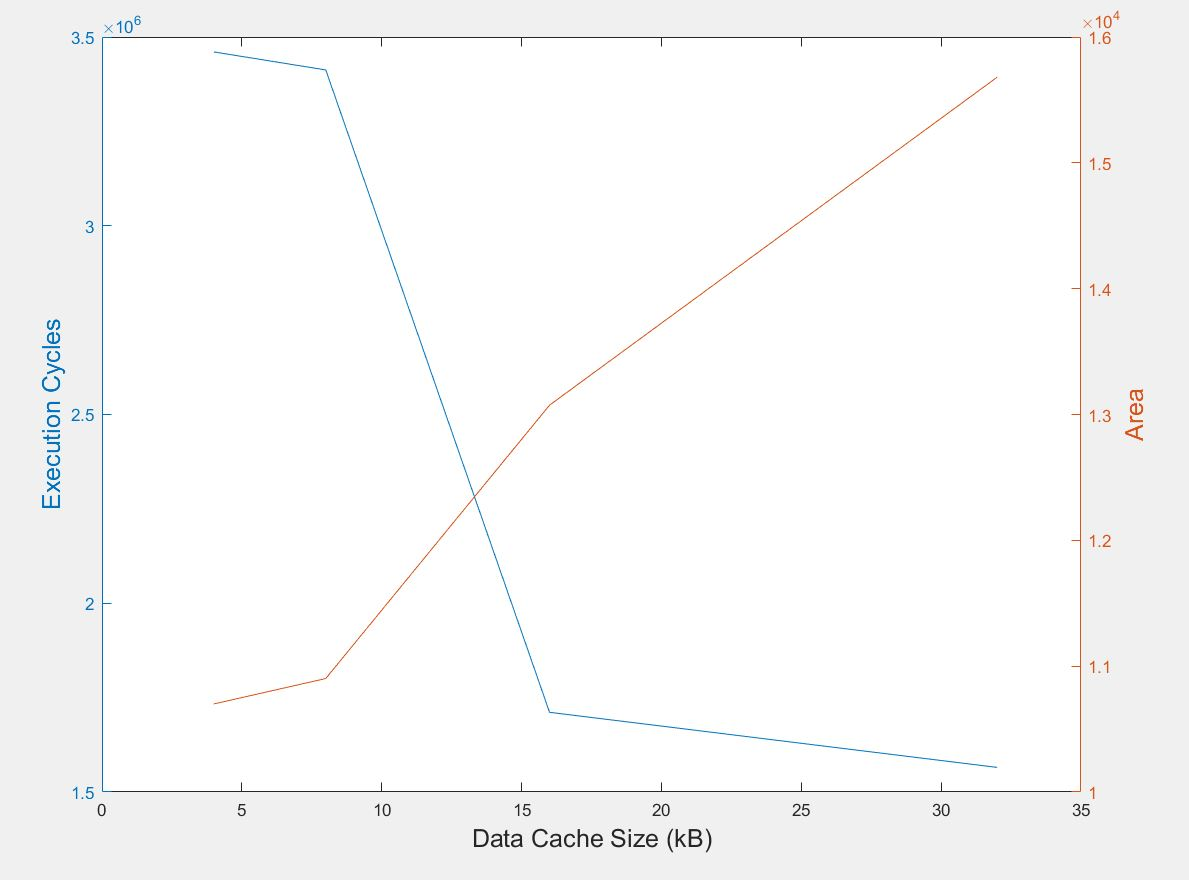
\includegraphics[width=3.6in]{CachePlot.JPG}
\caption{\label{fig:data} An example of how Data Cache size impacts Performance and Area Consumption (\textit{Matrix.c} with an 8-way core)}
\end{figure}

\subsection{Number of Stop Bits}
The stop bit functionality allows an improvement in performance by enabling the processor to execute a smaller number of instructions when NOPs are detected. Say, when a 4 issue width VLIW has 2 of the instructions to be executed as NOPs, the stop bit is set, which indicates that the remaining 2 instructions are NOPs and can be skipped. Instead, the processor can start executing the next 4-issue width instruction line. This functionality is especially useful in improving performance when dealing with larger issue width cores. The area increase when using stop bits is minimal since extra area is only needed for the logic circuitry to implement the stop bit functionality. The impact of using stop bits is illustrated in Figure 2. We notice a significant reduction in execution cycles but only a tiny increase in area.

We start our exploration on the basis of the above observations and then analyze the effect of varying the parameters on: (i) total no. of execution cycles, (ii) area, and (iii) energy consumption. We vary the issue width from 2 to 16, the number of cores, and the data and instruction cache sizes. The comparison of results for different configurations provides insights into how these affect performance, area and power consumption. For example, \textbf{we observe that the \textit{matrix} benchmark takes more executions cycles than the other benchmarks and is also significantly affected by the cache size. This, combined with our initial analysis, suggests that giving it an exclusive core, more multipliers, a higher issue width, and a larger cache is expected to improve the overall performance.}

\begin{figure}[h!]
\centering
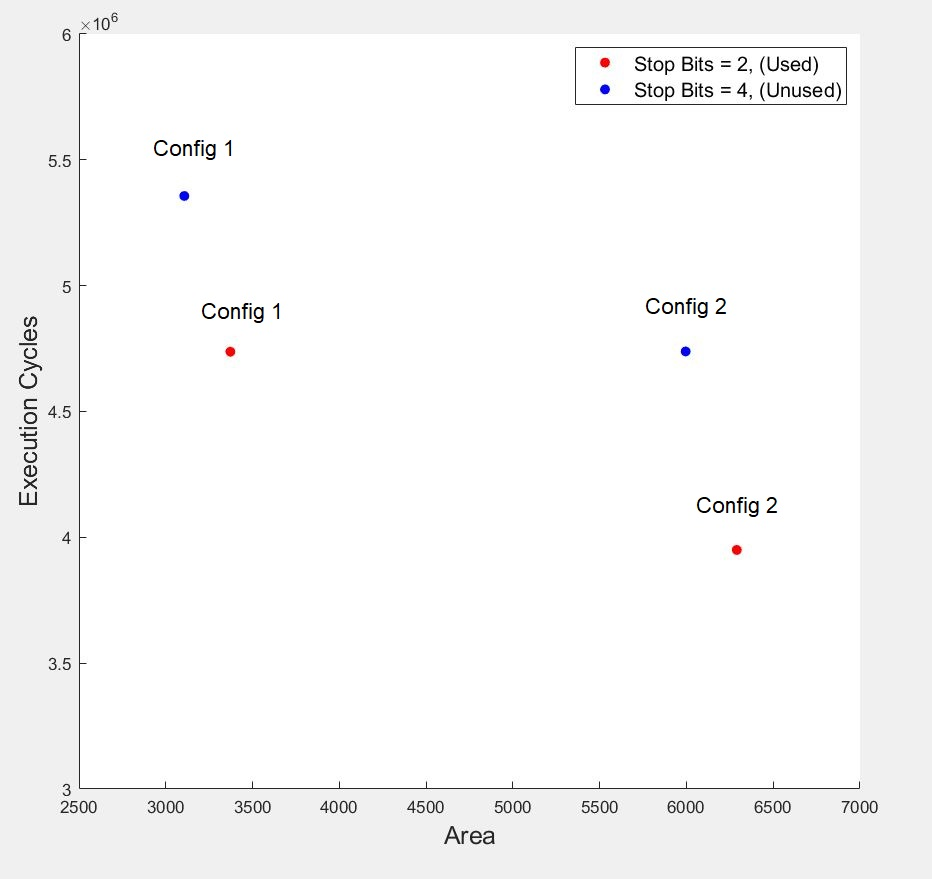
\includegraphics[width=3.6in]{StopBitPlot.JPG}
\caption{\label{fig:data} An example showing how usage of Stop bits for the same configuration leads to significant performance improvement while not increasing much.}
\end{figure}


\section{Design Configurations}

The main objective is to determine the best configuration(s) for each design approach: (i) performance maximization, (ii) energy minimization, and (iii) a balanced design with a good performance-energy-area trade-off. To achieve this, we create several configurations by varying the parameters discussed in the previous section. The analysis of each of the parameters separately and DSE results for individual benchmarks is used to group benchmarks with similar resource requirements together (especially in multi-core environments) for optimal utilization of resources. We start with the execution of all the benchmarks on a single static core and then move towards multi-core configurations in search of possibly better performances. Some of the configurations that were executed are included in Appendix I. The results of the runs are retrieved from the board server after running the designs on the FPGA bank.

We start with a given default configuration as follows:
\begin{itemize}
    \item Issue Width = 4
    \item No. of cores = 1
    \item No. of Multipliers = 4
    \item I\$ size= 16 KiB
    \item D\$ size= 4 KiB
    \item No stop bit (i.e. STOPBIT = 4)
\end{itemize}

The results of this configuration are:
\begin{itemize}
\item Total Execution Cycles: 4244362
\item Area: 4017.2
\item Energy: 2.2 mJ
\end{itemize}
This default configuration is considered the starting point reference for further optimization for each design approach.

\subsection{Configuration for Highest Performance}

The \textit{Matrix benchmark is the heaviest user of processor resources, followed by FIR. Convolution\_3x3 and CRC are comparatively smaller programs and require less resources for functioning}. We exploit this information for optimal distribution of resources - we start with (i) a 4-issue core exclusively for running Matrix with 4 multipliers, and (ii) another 4-way core for the rest of the benchmarks, also with 4 multipliers. 
To further improve the performance we proceed to a higher issue width of 8, with 8 multipliers for core0 running Matrix. As expected, this improves the performance but also increases the area; but in this design's motive, we consider only the performance numbers. Thus, for a better design, we add another core, ending up with the following optimum three-core design: 
\begin{enumerate}
    \item an 8-way Core0 running Matrix, with 4 multipliers, 
    \item a 4-way Core1 running FIR with the minimum number of multipliers (that is, 1), and
    \item a two-way Core2 for CRC and Convolution\_3X3, with two multipliers. 
\end{enumerate}

Increasing the issue width beyond 4 does not significantly increase the performance of Core1.
We observe that increasing both the instruction and data cache size from 16 KiB to 32 KiB for core0 significantly improves the performance. For core1, a instruction cache size of 16 KiB and Data Cache size of 4 is taken to be appropriate, since increasing it further, while improving core1's performance, does not affect the overall performance (it is lower bounded by the performance of \textit{Matrix} in core0). For instance, in one run, the number of execution cycles with D\$ = 4 KiB, I\$ = 16 KiB for FIR is 130,000. Increasing the cache to D\$ = 8 KiB, I\$ = 32 KiB decreases the cycle count to 110,000. But the number of execution cycles for Matrix (around 160,000) determines the overall performance. Core2 is given 8 KiB of I\$ and 4 KiB of D\$ since the CRC and Convolution benchmarks are small programs which exhibit good performance even with limited resources. Finally, providing 2 stop bits to each of the cores results in a significant decrease in the number of execution cycles as opposed to a higher number.

\begin{figure}[h!]
\centering
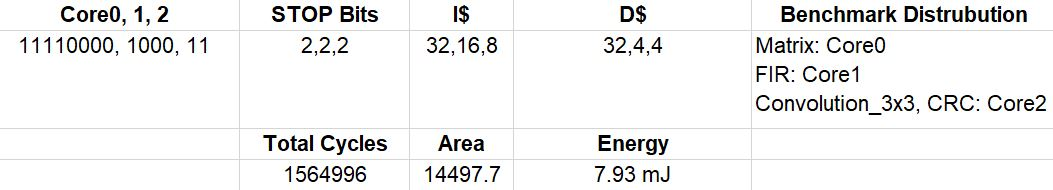
\includegraphics[width=3.5in]{HighPerf.JPG}
\caption{\label{fig:data}High Performance Configuration }
\end{figure}

\subsection{Configuration for Low Power Consumption}

The aim of this approach is to minimize the FPGA area utilized and energy consumed without a significant degradation of performance.\\
Starting with the default configuration, we perform the following steps to arrive at an optimum configuration for low power consumption.
\begin{itemize}
    \item We first reduce the data and instruction cache size by half to 2 KiB and 8 KiB respectively; however, this improves the area only slightly. We set STOPBIT = 2. This improves the performance significantly without increasing the area too much.
    \item We analyze the energy, area and performance results employing 2 cores (11,11) both having 2 multipliers each and both cores having 16 KiB of I\$ and 4 KiB of D\$. We observe that the area increases too much and also the performance degrades significantly. The reason for this result for the configuration is that since matrix benchmark is a large program, it requires a high issue width and a large number of multipliers.
    \item Hence, keeping in mind the above observation, we go with a single core, and optimize the no. of multipliers and cache size for minimal power consumption. We arrive at the following result: a four-way single Core design with three multipliers.

\end{itemize}

\begin{figure}[h!]
\centering
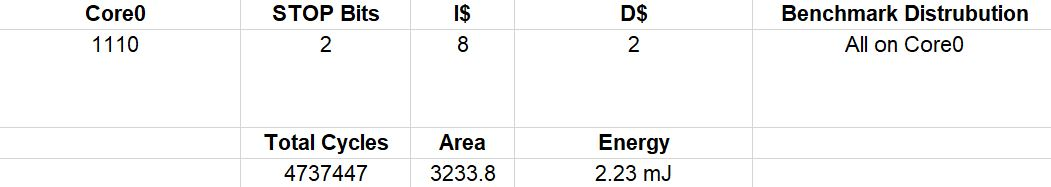
\includegraphics[width=3.5in]{LowPower.JPG}
\caption{\label{fig:data} Low Power Configuration }
\end{figure}
\begin{figure}[h!]
\centering
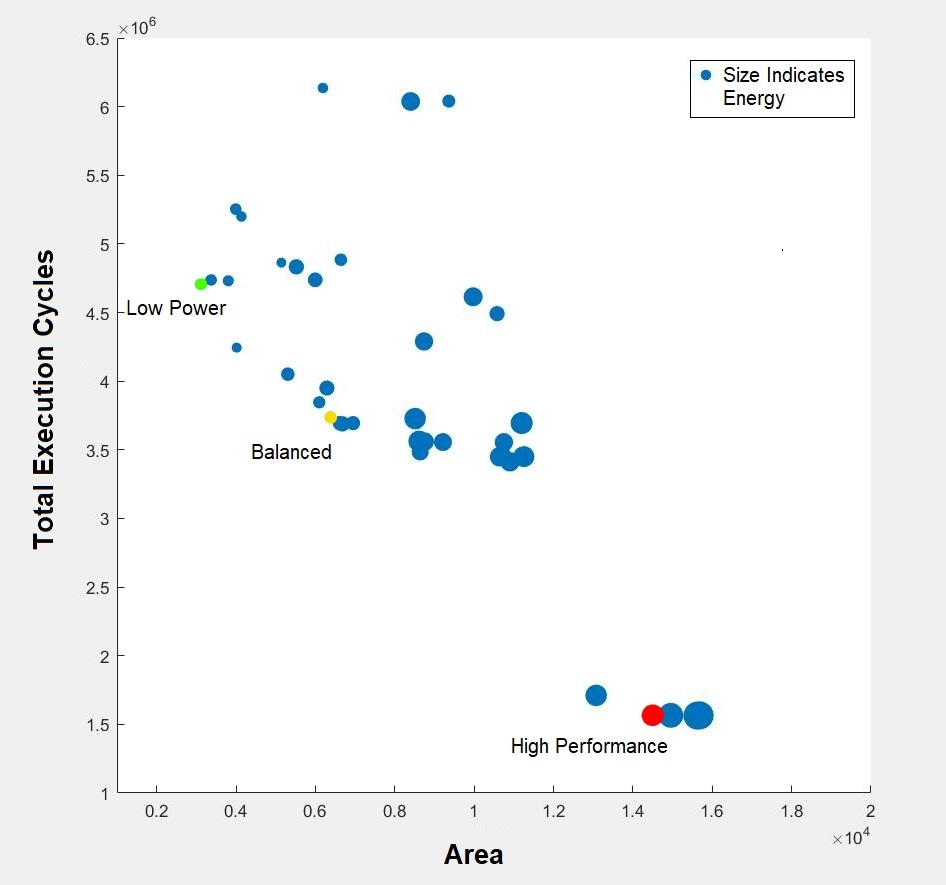
\includegraphics[width=3.6in]{FinalPlot.jpg}
\caption{\label{fig:data} \textbf{Overall Design Space Exploration}. Size of the circles indicates Energy consumption. The chosen configurations for Low Power, High Performance and Balanced Design are highlighted.}
\end{figure}

\subsection{Energy-Area-Performance Compromise}

We use the results of our overall Design Space Exploration (shown in Figure 5) to arrive at a well balanced design.

We notice for this Overall DSE plot (Figure 5) how performance improvement comes at the cost of area increase. Moreover, we also notice how energy consumed and area utilized are closely correlated since the size of the circles (indicating Energy) increases as we move from the left to the right of the plot (increasing area).

The well balanced design is chosen with the objective of achieving a reasonable performance while not increasing the area too much.
For this, we finally choose a 2 core design with \textit{Matrix} occupying one core while the rest of the benchmarks (which are smaller) occupying the other core. Issue width for \textit{Matrix} is kept at 4 and the number of multipliers for this issue width is maximized for the balanced design.
We arrive at the following result:
\begin{itemize}
    \item a 4-way Core0 running Matrix, with 4 multipliers,
    \item a 4-way Core1 running FIR, Convolution\_3x3 and CRC with 2 multipliers.
\end{itemize}
Reasonable performance is reached with a Cache Size of 8 KiB and 4 KiB (Instruction and Data) for core0 and smaller cache sizes for core1 (8 and 2 KiB respectively).

\begin{figure}[h!]
\centering
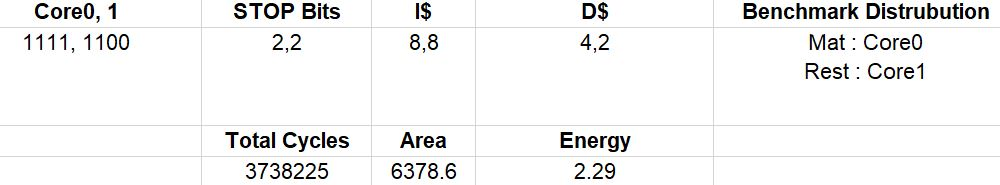
\includegraphics[width=3.5in]{Balanced.JPG}
\caption{\label{fig:data} Balanced Design Configuration }
\end{figure}

\begin{comment}
Final Remarks:
\begin{itemize}

\item Used stop bits especially with larger issue width which we will have here since we are trying to maximize perf--significant improvement in perf  without inc area too much
\item degrading any core in terms of resources too drastically leads to sig no of stalls which leads to stalls in overall execution, exec time shots up which we dont want
 \item so we tried to opt the cores and made sure each core had sign no. of res so as to npt create too many stalls
    \item so we ended up with this final config for best perf.
    \item 
\end{itemize}

\section{Proposal for well-balanced design and related measurement results.}

Discuss your results. Compare the two values of $n_{s}$ that you've found in the previous section. Compare your results with literature and comment on the difference. If you didn't know the value of the resistance quantum, would you be able to deduce it from your measurements? If yes/no, why?
\end{comment}

\section{Conclusions and Chosen Design for the 4 Applications' domain}

The Matrix benchmark is the main bottleneck in the workload since in the default configuration it does not get the resources it needs. After adding more resources (multipliers, I- and D-cache, increasing the issue width) and assigning a core exclusively to it, we see that the performance increases by about 50 \%. However, the area increases as well since the additional components require a lot of FPGA slices.
The other applications require far less in terms of hardware resources, and hence needn't have exclusive cores each. Our decisions to allot cores were made accordingly.\\
Overall, we see how changing the various parameters can greatly affect the results based on the approach taken (for instance, for maximizing performance, the area increase wasn't taken into consideration in the decisions, whereas for area minimization, the impact on performance wasn't considered.)\\
We thus conclude that choosing a configuration ultimately depends on the intended use case(s).\textit{ The applications provided to us (matrix, FIR, CRC and convolution) are all related to communication and signal (image) processing, and probably are ones that run in embedded processors in handheld cameras, cellphones, and the like. Though our High performance configuration minimizes the execution cycles in an optimal way, its area is high and its I\$ and D\$ numbers of 32 each are unrealistic for such a scenario. Thus, the performance-energy-area compromise design seems best suited for the four applications.}

\begin{comment}
1. matrix needs a lot of cache (bottleneck in the workload)
2. increasing cache size of data and Instruction caches improves performance
4. no. of execution cycles decreases(almost half) for matrix.c on increasing the size of instruction cache.
3. area of slices significantly increases on increasing cache size
\end{comment}
\label{sec:latex}
\section{Reflection: Learnings from this Assignment}

This assignment introduced us to the process of choosing hardware resources keeping in mind the requirements of an application (or multiple applications in parallel) intended to be run on a processor, and the impact of varying the parameters associated with it. It also got us familiarized with the reasoning behind the splitting of a processor into multiple cores, and how power savings and performance improvements can be achieved with simple tweaks to the configuration parameters. Moreover, we also learned that performance almost always comes at a cost beyond a certain point of resource optimization, in the form of increased area and/or energy usage. We now know that parallelization is not as straightforward as it may initially seem since it requires thinking from a different paradigm and perspective and depends heavily on the processor of allotting resources to cores, and on the applications as well. Hence it is necessary to gauge the applications' requirements and the design constraints through analyses and simulations before synthesizing the hardware as otherwise a lot of extra time and effort would be consumed. It was a good, hands-on, learning experience in computer engineering, given that we actually synthesized processors on FPGAs and ran applications on them.
\newpage
\section{Appendix}
List of important configurations:\\
\begin{figure}[h!]
\centering
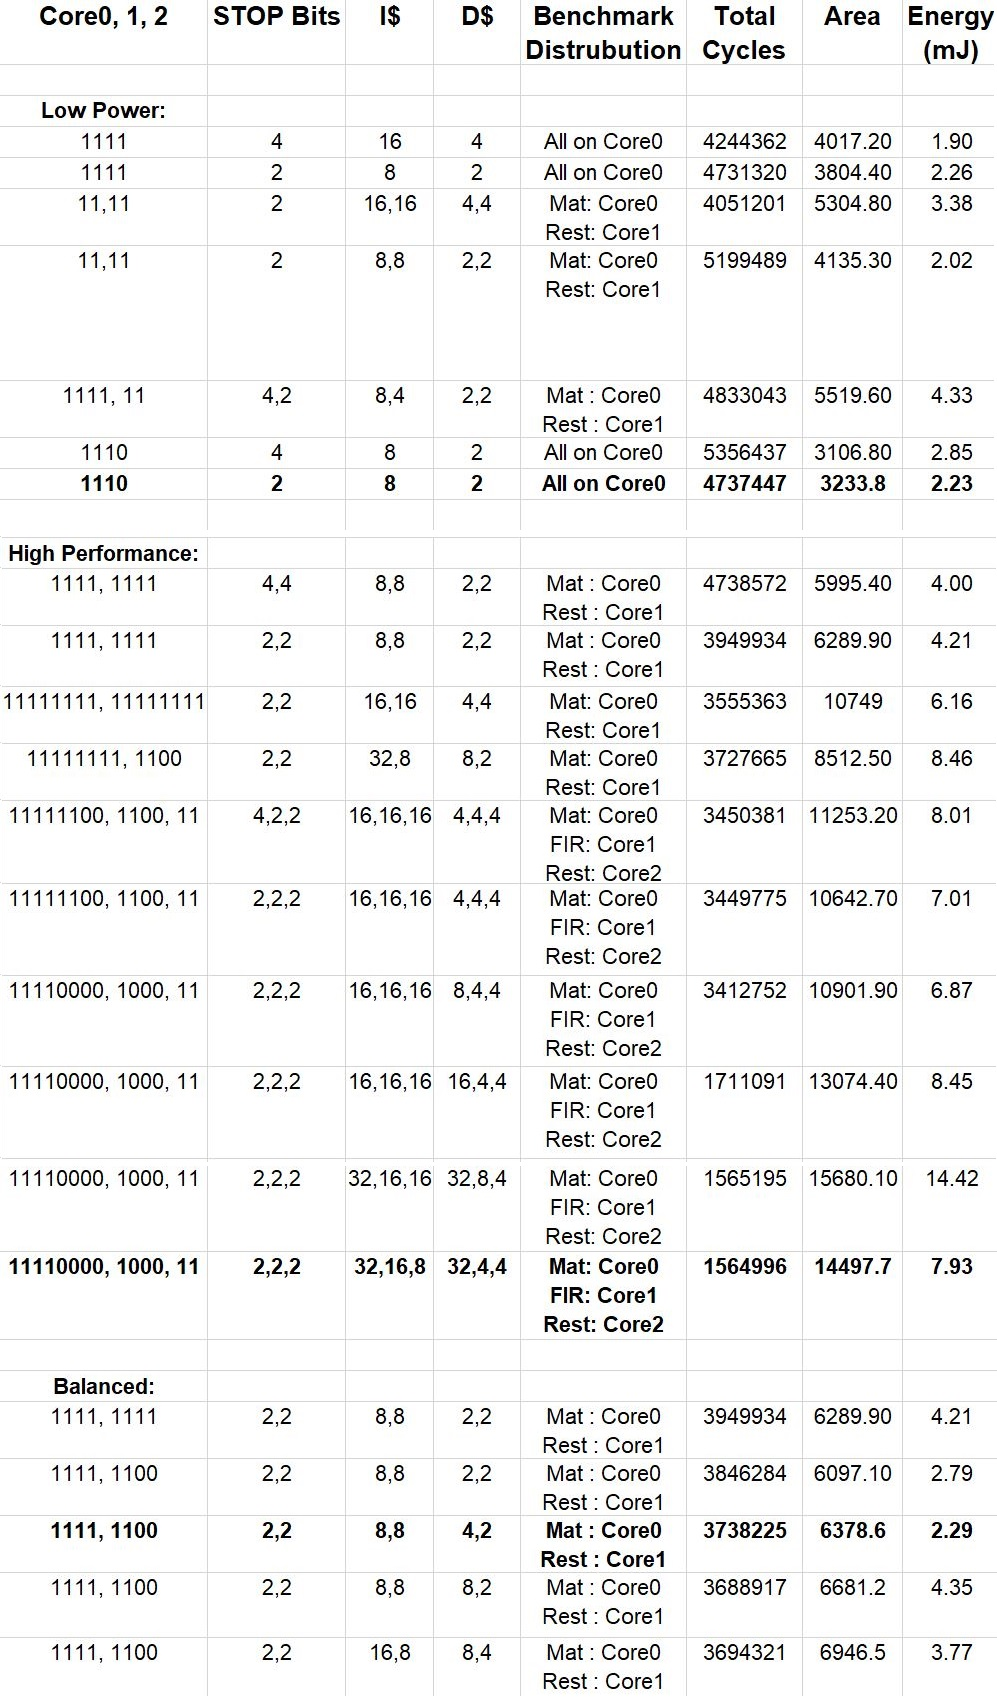
\includegraphics[width=3.5in]{Appendix.jpg}
%\caption{\label{fig:data} Balanced Design Configuration }
\end{figure}
\begin{comment}
First you have to upload the image file (JPEG, PNG or PDF) from your computer to writeLaTeX using the upload link the project menu. Then use the includegraphics command to include it in your document. Use the figure environment and the caption command to add a number and a caption to your figure. See the code for Figure \ref{fig:frog} in this section for an example.
\end{comment}


\end{document}